% !TeX root = ../main.tex
% Add the above to each chapter to make compiling the PDF easier in some editors.

\chapter{Congruence Closure} \label{chapter:congruence_closure}

Congruence closure considers equations containing constants and function symbols. Each function symbol is associated with an arity, which is the number of parameters it accepts. The congruence closure $CC(S)$ of a set of equations $S$ is the smallest reflexive, symmetric, transitive and monotonic superset of the equations. It is inductively defined as follows \cite{congruenceclosure-ac}:

\begin{enumerate}[label=(\roman*)]
\itemsep0em
    \item $S \subseteq CC(S)$.
    \item $\forall a: a = a \in CC(S)$ (reflexivity).
    \item if $a = b \in CC(S)$, then $b = a \in CC(S)$ (symmetry).
    \item if $a = b \in CC(S)$ and $b = c \in CC(S)$, then $a = c \in CC(S)$ (transitivity).
    \item $\forall f$ of arity $k :$ if $\forall i \in [1..k]: a_i = b_i \in CC(S)$, then $f(a_1, ..., a_k) = f(b_1,..., b_k) \in CC(S)$ (monotonicity).
\end{enumerate}

This chapter describes the implementation of an algorithm which maintains the congruence closure of a set of equations.
The algorithm was described by Nieuwenhuis and Oliveras \cite{Nieuwenhuis}.

Similarly to the union-find algorithm, the congruence closure algorithm starts with an empty data structure. It supports the following two functions:
\begin{itemize}
    \item \lstinline|merge|: adds one additional equation to the data structure.
    \item  \lstinline|are_congruent|: returns \emph{True} if a given equation is contained in the congruence closure.
\end{itemize}

The data structure contains a union-find forest, in order to maintain the equivalence classes of the variables. Additionally, there is another forest, called the \emph{proof forest}. It is similar to the union-find forest as it maintains the same equivalence classes, but it differs in the positioning of the edges.
Moreover, it contains two data structures for storing equations containing function symbols. The following sections describe the \emph{proof forest} and then the congruence closure algorithm, as well as their correctness proofs.

As before, the optimizations of path compression and union by rank are left out. These optimizations are not relevant for the correctness of the algorithm, and they could later be added to a refinement of the algorithm.

\section{Input Equations}\label{section:inputequations}

Arbitrary equations can be transformed to equations which have one of the following two forms: either constant equations of the form $a = b$ or equations of the form $F(a,b) = c$, where $a$, $b$ and $c$ are constants from a set of $n$ constants, which are indexed from $0$ to $n-1$. $F$ is a specific function of arity 2.

The transformation is done by currying and by introducing new constant symbols. For a detailed explanation of how this is done, refer to \cite{Nieuwenhuis2}. In order to understand this thesis, it is irrelevant to know how the transformation is done.
The congruence closure of the transformed equations is equal to the congruence closure of the original equations \cite{Nieuwenhuis2}, therefore in the following, we will only consider the transformed equations.
The datatype used for these equations is the one described in Subsection \ref{subsubsection:datatypes}.

\section{Congruence Closure Implementation}

\subsection{The Proof Forest}

In order to implement a \emph{cc\_explain} operation efficiently, the paper by Nieuwenhuis et al. \cite{Nieuwenhuis} introduces an additional data structure, the \emph{proof forest}. It is a forest which has as nodes the variables and as edges the unions that were made. Each time \lstinline|ufa_union| is called on the union-find forest, the proof forest is modified with \lstinline|add_edge|. In order to avoid the creation of cycles, redundant unions are ignored.

\subsubsection{add\_edge}
\label{subsubsection:addedge}

Analogously to the union-find forest, the proof forest has directed edges and for each equivalence class there is a representative element, or root. We denote the root of an element $x$ in the proof forest $pf$ as $rep\_of(pf, x)$. All edges are directed towards the root. To keep this invariant, each time an edge from $x$ to $y$ is added, all the edges on the path from $rep\_of(pf, x)$ to $x$ are reversed.
In the implementation, the proof forest is represented by a list, which stores the parent of each node, exactly as in the union-find list. As before, the parent of an element $x$ in the proof forest $pf$ is denoted as $pf ! x$. The implementation for adding an edge, which corresponds to the \lstinline{union} operation, is the following:

\begin{lstlisting}
function (domintros) add_edge :: "nat list ⇒ nat ⇒ nat ⇒ nat list"
  where
"add_edge pf x y = (if pf ! x = x
                        then (pf[x := y])
                        else add_edge (pf[x := y]) (pf ! x) x)"
  by pat_completeness auto
\end{lstlisting}

\begin{exmp}
Assuming the proof forest looks like this

\begin{center}
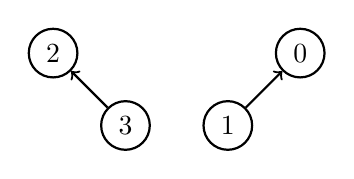
\begin{tikzpicture}[node distance={13mm}, thick, main/.style = {draw, circle}]
\node[main] (0) {0};
\node[main] (1) [below left of=0] {1};
\node[main] (3) [left of=1] {3};
\node[main] (2) [above left of=3] {2};

\draw[->] (3) -- (2);
\draw[->] (1) -- (0);
\end{tikzpicture}
\end{center}

After adding an edge between 3 and 1, the edges from 3 to its root 2 are inverted.

\begin{center}
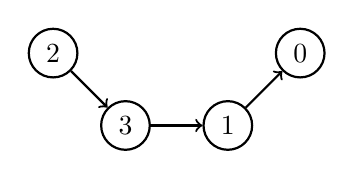
\begin{tikzpicture}[node distance={13mm}, thick, main/.style = {draw, circle}]
\node[main] (0) {0};
\node[main] (1) [below left of=0] {1};
\node[main] (3) [left of=1] {3};
\node[main] (2) [above left of=3] {2};

\draw[->] (2) -- (3);
\draw[->] (3) -- (1);
\draw[->] (1) -- (0);
\end{tikzpicture}
\end{center}
\end{exmp}

We can show that \lstinline{add_edge pf x y} terminates, if the invariant \lstinline{ufa_invar} holds for the proof forest and $x$ and $y$ do not belong to the same equivalence class.

\begin{lstlisting}
lemma add_edge_domain:
  assumes "ufa_invar pf" "rep_of pf x ≠ rep_of pf y"
  shows "add_edge_dom (pf, x, y)"
\end{lstlisting}

\begin{proof}
It can be proven by induction on the length of the path $p$ from $rep\_of(pf, x)$ to $x$.

In the base case there is only one node in the path, hence $x$ must be equal to its root, therefore $pf ! x = x$ and the algorithm terminates immediately.

In the other case $x$ is not a root. This implies that there is a path $p'$ from $rep\_of(pf,x)$ to $pf!x$ which is shorter than the path from $rep\_of(pf,x)$ to $x$. The path $p'$ is also present in the $pf[x := y]$, because the path does not contain $x$. Also, the representative of $x$ in $pf[x := y]$ is equal to the representative of $y$, and $rep\_of(pf[x := y],pf!x)$ is still equal to the old representative $rep\_of(pf,pf!x)$, therefore they are not in the same representative class, and we can apply the induction hypothesis and conclude that the recursive call terminates, therefore the function terminates.
\end{proof}

In order to prove the correctness of \lstinline|add_edge|, we show that \lstinline{ufa_union l x y} and \lstinline{add_edge l x y} have the same behaviour.
We can conclude from this that the equivalence classes of the union-find forest are the same as those of the proof forest.
The theory \lstinline{Union_Find} from the AFP \cite{Sep} already provides the following lemma for \lstinline{ufa_union}:

\begin{lstlisting}
lemma ufa_union_aux:
  "rep_of (ufa_union l x y) i =
    (if rep_of l i = rep_of l x then rep_of l y else rep_of l i)"
\end{lstlisting}

We can show a similar lemma for \lstinline{add_edge}.
The additional assumption \lstinline{rep_of pf x ≠ rep_of pf y} does not cause problems, because \lstinline{add_edge} is only executed by the congruence closure algorithm when \lstinline{rep_of pf x ≠ rep_of pf y}.

\begin{lstlisting}
lemma rep_of_add_edge_aux:
   assumes "rep_of pf x ≠ rep_of pf y"
   shows "rep_of (add_edge pf x y) i =
     (if rep_of pf i = rep_of pf x then rep_of pf y else rep_of pf i)"
\end{lstlisting}

\begin{proof}
We already showed that the function terminates, therefore we can prove it by computation induction on \lstinline{add_edge}.
\end{proof}

We also show that \lstinline|add_edge| reverses all the edges from $rep\_of(pf,x)$ to $x$, and it adds an edge from $x$ to $y$, i.e., after \lstinline|add_edge| the forest contains a path from $y$ to $rep\_of(pf,x)$. This path is the original path from $rep\_of(pf,x)$ to $x$ reversed and with one edge added between $x$ and $y$. \lstinline|rev| is a function which reverses a list, and \lstinline|path_to_root| is the function described in Subsection \ref{subsubsection:path-to-root}. The proof can be shown by computation induction on \lstinline|add_edge|.

\begin{lstlisting}
lemma add_edge_correctness:
  assumes "ufa_invar pf"
    "rep_of pf x ≠ rep_of pf y"
  shows
  "path (add_edge pf x y) y ([y] @ rev (path_to_root pf x)) (rep_of pf x)"
\end{lstlisting}

The proof forest has a similar structure as the union-find forest, therefore we prove that \lstinline|add_edge| preserves the \lstinline|ufa_invar| invariant from Section \ref{section:uf-isabelle}. This allows us to apply all the lemmas that were proven for the union-find forest also to the proof forest.

\begin{lstlisting}
lemma add_edge_ufa_invar_invar:
  assumes "ufa_invar pf"
    "rep_of pf x ≠ rep_of pf y"
  shows "ufa_invar (add_edge pf x y)"
\end{lstlisting}

\begin{proof}
First, we prove that the invariant holds after a function update, if the update does not cause the formation of a cycle. Then we show that each function update of \lstinline|add_edge| does not form a cycle.
\end{proof}

\subsubsection{add\_label}
\label{subsubsection:addlabel}

Additionally, each edge is labeled with the input equation, or the input equations, which caused the adding of this edge. This is not necessary for the congruence closure algorithm by itself, but it will be needed by the \emph{cc\_explain} operation.
There are two possible types of labels: either one equation $a = b$, or two equations of the type $F(a_1, a_2) = a$ and $F(b_1, b_2) = b$, where $a_1$ and $b_1$ as well as $a_2$ and $b_2$ were already in the same equivalence class before this union.
Both these cases can cause the union between the equivalence classes of $a$ and $b$.
The labeling is implemented by using an additional list, called \lstinline|pf_labels|.
It contains at each index the label of the outgoing edge, or \lstinline|None| if there is no outgoing edge.
It is similar to the \emph{associated unions} list of union-find, but it contains the labels directly, instead of an index to another list.

The labels have the type \lstinline|pending_equation|, which can be either one or two equations. The name \lstinline|pending_equation| derives from the fact that it is also the type of the elements of the \lstinline|pending| list, which will be described in the next section. The datatype is defined as follows:

\begin{lstlisting}
datatype pending_equation = One equation
  | Two equation equation
\end{lstlisting}

Theoretically this allows also for invalid equations, for example, two equations of the type $a = b$ and $c = d$, but we will prove in the next sections that the equations in the \lstinline|pf_labels| list are always either \lstinline{One} ($a = b$) or \lstinline{Two} ($F(a_1, a_2) = a$) ($F(b_1, b_2) = b$).

Each time an edge gets added to the \emph{proof forest}, the labels need to be updated as well. The function \lstinline{add_label} adds a label to the new edge, and modifies the labels for the edges which are reversed by \lstinline{add_edge}. \lstinline|pfl| represents the \lstinline|pf_labels| list.

\begin{lstlisting}
function (domintros) add_label :: "pending_equation option list ⇒ nat list ⇒ nat ⇒ pending_equation ⇒ pending_equation option list"
  where
"add_label pfl pf x lbl =
    (if pf ! x = x
        then (pfl[x := Some lbl])
        else add_label (pfl[x := Some lbl]) pf (pf ! x) (the (pfl ! x)))"
  by pat_completeness auto
\end{lstlisting}

Similarly to the \lstinline{path_to_root} function, \lstinline{add_label} has the same recursive calls as \lstinline{rep_of}, therefore it has the same domain.

\begin{lstlisting}
lemma rep_of_dom_iff_add_label_dom:
  "rep_of_dom (pf, y)  ⟷  add_label_dom (pfl, pf, y, y')"
\end{lstlisting}

\subsection{Congruence Closure Data Structure}
\label{subsection:datastructure}

For the congruence closure algorithm there are five important data structures, which are described in the following. More details on this topic can be found in \cite{Nieuwenhuis}.

\begin{itemize}
	\item \lstinline{cc_list}: the union-find list, corresponds to the \lstinline{uf_list}.

	\item \lstinline{use_list}: a two-dimensional list which contains for each index $a$ a list of input equations $F(b_1, b_2) = b$ where the representative of $b_1$ or $b_2$ is $a$.
    Only indexes which symbolize representative elements contain equations.

	\item \lstinline{lookup}: The purpose of this table is to store a model equation for each pair of representatives. It is indexed by pairs of representatives $b$ and $c$. At index $(b,c)$ it stores an input equation $F(a_1, a_2) = a$, such that $b$ is the representative of $a_1$ and $c$ is the representative of $a_2$, or \lstinline{None} if no such equation exists.

    \item \lstinline{pending}: equations of the type \lstinline{One} ($a = b$) or \lstinline{Two} ($F(a_1, a_2) = a$) ($F(b_1, b_2) = b$) where $a$ and $b$ need to be merged, and $a_1$ and $b_1$ as well as $a_2$ and $b_2$ are already in the same congruence class.

    \item \lstinline{proof_forest}: the proof forest as described in Subsection \ref{subsubsection:addedge}.

    \item \lstinline{pf_labels}: the labels of the proof forest as described in Subsection \ref{subsubsection:addlabel}.

    \item \lstinline{input}: a set of the input equations, which will be useful for some proofs in the next sections.
\end{itemize}

In the following, we shall refer to \lstinline{cc_list} as $l$, the use list as $u$, the lookup table as $t$, the pending list as $pe$, the proof forest as $pf$, the labels list for the proof forest as $pfl$ and the input as $ip$, unless otherwise stated.

\subsection{Congruence Closure Algorithm}

With this data structure we can implement the \lstinline{merge} function as described in \cite{Nieuwenhuis}.
It takes as parameter the current congruence closure data structure and an equation, which it adds to the data structure. The \lstinline{propagate} function used by \lstinline{merge} will be described later. It performs unions between the constant symbols in the pending list.

If the input equation is of the type $a = b$, then the equation is added to \lstinline|pending|. The \lstinline|propagate| function then merges the equivalence classes of $a$ and $b$.

If the input equation is of the type $F(a_1, a_2) = a$, then there are two possibilities: if there is already an equation $F(b_1, b_2) = b$ in the lookup table at the index $(rep\_of(l,a_1), rep\_of(l,a_2))$, then we know that $a_1 = b_1$ and $a_2 = b_2$. Therefore, we add $F(b_1, b_2) = b$ and $F(a_1, a_2) = a$ to pending, so that the equivalence classes of $a$ and $b$ will be merged by \lstinline|propagate|.
On the other hand, if the respective lookup entry is \lstinline{None}, then the equation is added to the lookup table at the index $(rep\_of(l,a_1), rep\_of(l,a_2))$, so that the next time an equation with congruent parameters is input, they will be added together to pending.

For this case distinction there are two auxiliary functions.
The function \lstinline{lookup_Some} returns \emph{True} if there is an entry in lookup at the index $(rep\_of(l,a_1), rep\_of(l,a_2))$ and \emph{False} otherwise. The function \lstinline{update_lookup} adds the equation to lookup at the index $(rep\_of(l,a_1), rep\_of(l,a_2))$.

The following is the implementation of \lstinline|merge| in Isabelle.


\begin{lstlisting}
fun merge :: "congruence_closure ⇒ equation ⇒ congruence_closure"
  where
"merge ⦇cc_list = l, use_list = u, lookup = t, pending = pe, proof_forest = pf, pf_labels = pfl, input = ip⦈
(a ≈ b) =
  propagate
    ⦇cc_list = l, use_list = u, lookup = t, pending = One (a ≈ b)#pe, proof_forest = pf, pf_labels = pfl, input = insert (a ≈ b) ip⦈"
| "merge ⦇cc_list = l, use_list = u, lookup = t, pending = pe, proof_forest = pf, pf_labels = pfl, input = ip⦈
(F a$_1$ a$_2$ ≈ a) =
(if (lookup_Some t l (F a$_1$ a$_2$ ≈ a))
  then propagate ⦇cc_list = l, use_list = u, lookup = t,
            pending = link_to_lookup t l (F a$_1$ a$_2$ ≈ a)#pe,
            proof_forest = pf, pf_labels = pfl, input = insert (F a$_1$ a$_2$ ≈ a) ip⦈
  else ⦇cc_list = l,
          use_list = (u[rep_of l a$_1$ := (F a$_1$ a$_2$ ≈ a)#(u ! rep_of l a$_1$)])
          [rep_of l a$_2$ := (F a$_1$ a$_2$ ≈ a)#(u ! rep_of l a$_2$)],
          lookup = update_lookup t l (F a$_1$ a$_2$ ≈ a),
          pending = pe, proof_forest = pf, pf_labels = pfl,
          input = insert (F a$_1$ a$_2$ ≈ a) ip⦈
)"
\end{lstlisting}

The main part of the algorithm is executed in \lstinline{propagate}. It recursively takes one item from pending and performs the union of the representative classes. As previously mentioned, the pending item could be either an equation of the type $a = b$, or two equations of the type $F(a_1, a_2) = a$ and $F(b_1, b_2) = b$, where $a_1$ and $a_2$ are already in the same representative class as $b_1$ and $b_2$ respectively. In both cases the representative classes of $a$ and $b$ need to be merged.

\begin{lstlisting}
function propagate :: "congruence_closure ⇒ congruence_closure"
  where
"propagate ⦇cc_list = l, use_list = u, lookup = t, pending = [], proof_forest = pf, pf_labels = pfl, input = ip⦈ =
⦇cc_list = l, use_list = u, lookup = t, pending = [], proof_forest = pf, pf_labels = pfl, input = ip⦈"
| "propagate
⦇cc_list = l, use_list = u, lookup = t, pending = (eq # pe), proof_forest = pf, pf_labels = pfl, input = ip⦈ =
(let a = left eq; b = right eq in
  (if rep_of l a = rep_of l b
    then propagate ⦇cc_list = l, use_list = u, lookup = t, pending = pe, proof_forest = pf, pf_labels = pfl, input = ip⦈
    else
      propagate (propagate_step l u t pe pf pfl ip a b eq))
)"
  by pat_completeness auto
\end{lstlisting}

The functions \lstinline{left} and \lstinline{right} simply retrieve $a$ and $b$ from either of the two types of pending equations. If $a$ and $b$ are already in the same representative class, nothing needs to be done, otherwise the union is performed. For more clarity, the union is defined separately as \lstinline{propagate_step}.


The union consists of \lstinline{ufa_union}, \lstinline{add_edge} and \lstinline{add_label}, as well as the function \lstinline|propagate_loop| which moves all elements from the use list of $rep\_of(l,a)$ to either $rep\_of(l, b)$, or to pending. This is necessary, because the old representative of $a$ is not a representative any more, and its new representative is  $rep\_of(l, b)$.

\begin{lstlisting}
abbreviation propagate_step
  where
"propagate_step l u t pe pf pfl ip a b eq ≡
  propagate_loop (rep_of l b) (u ! rep_of l a)
    ⦇cc_list = ufa_union l a b,
    use_list = u[rep_of l a := []],
    lookup = t,
    pending = pe,
    proof_forest = add_edge pf a b,
    pf_labels = add_label pfl pf a eq,
    input = ip⦈"
\end{lstlisting}

The \lstinline|propagate_loop| is defined as a recursive function. It considers each element of the use list of $rep\_of(l, a)$, and either adds it to the use list of $rep\_of(l, b)$ and the lookup table, or, if there is already an entry in lookup, then that entry together with the current equation are added to pending.

\begin{lstlisting}
fun propagate_loop
  where
"propagate_loop rep_b (u1 # urest)
⦇cc_list = l, use_list = u, lookup = t, pending = pe, proof_forest = pf, pf_labels = pfl, input = ip⦈
=
  propagate_loop rep_b urest (
    if (lookup_Some t l u1)
    then
      ⦇cc_list = l, use_list = u, lookup = t,
            pending = link_to_lookup t l u1#pe,
            proof_forest = pf, pf_labels = pfl, input = ip⦈
    else
      ⦇cc_list = l,
            use_list = u[rep_b := u1 # (u ! rep_b)],
            lookup = update_lookup t l u1,
            pending = pe, proof_forest = pf, pf_labels = pfl, input = ip⦈
)"
| "propagate_loop _ [] cc = cc"
\end{lstlisting}

\begin{exmp}\label{example:merge}
Let $cc$ be a congruence closure data structure with an empty use list and lookup, with a union-find list $l$ and with the following proof forest. Only the indexes 0 and 2 are shown in the tables, because the other elements are not representatives.


\begin{table}[!htb]
    \centering
    \begin{tabular}{ c c }
        \begin{tabular}{ c }
            \emph{proof forest}\\
            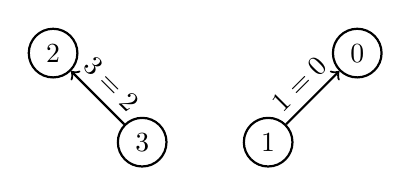
\begin{tikzpicture}[baseline=0, node distance={16mm}, thick, main/.style = {draw, circle}]
            \node[main] (0) {0};
            \node[main] (1) [below left of=0] {1};
            \node[main] (3) [left of=1] {3};
            \node[main] (2) [above left of=3] {2};

            \draw[->] (3) -- node[midway, above, sloped]{$3 = 2$} (2);
            \draw[->] (1) -- node[midway, above, sloped]{$1 = 0$} (0);
            \end{tikzpicture}
        \end{tabular}
    &
        \begin{tabular}{ c }
            \emph{use list}\\
            \begin{tabular}{ |c|c| }
                \hline
                index & use list \\
                \hline
                0 & [] \\
                \hline
                2 & [] \\
                \hline
           \end{tabular}
        \end{tabular}
        \begin{tabular}{ c }
            \emph{lookup table}\\
            \begin{tabular}{ |c|c|c| }
                \hline
                    & 0 & 2 \\
                \hline
                0 & None & None \\
                \hline
                2 & None & None \\
                \hline
            \end{tabular}
         \end{tabular}
    \end{tabular}
\end{table}


This shows that 2 and 3 are in one equivalence class and 1 and 0 are in the other.

If we apply \lstinline{merge} with the equation $F(0,2) = 1$, then the algorithm considers the lookup entry at the index $(rep\_of(l, 0), rep\_of(l, 2)) = (0,2)$, which is empty, therefore the equation is added to the use list and to lookup. The data structure then looks like this:

\begin{table}[!htb]
    \centering
    \begin{tabular}{ c c }
        \begin{tabular}{ c }
            \emph{proof forest}\\
            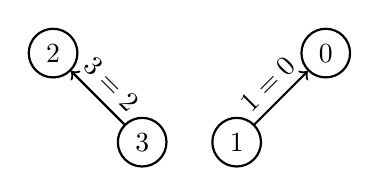
\begin{tikzpicture}[baseline=0, node distance={16mm}, thick, main/.style = {draw, circle}]
            \node[main] (0) {0};
            \node[main] (1) [below left of=0] {1};
            \node[main] (3) [left of=1, node distance=12mm] {3};
            \node[main] (2) [above left of=3] {2};

            \draw[->] (3) -- node[midway, above, sloped]{$3 = 2$} (2);
            \draw[->] (1) -- node[midway, above, sloped]{$1 = 0$} (0);
            \end{tikzpicture}
        \end{tabular}
    &
        \begin{tabular}{ c }
            \emph{use list}\\
            \begin{tabular}{ |c|c| }
                \hline
                index & use list \\
                \hline
                0 & [$F(0,2) = 1$] \\
                \hline
                2 & [$F(0,2) = 1$] \\
                \hline
           \end{tabular}
        \end{tabular}
        \begin{tabular}{ c }
            \emph{lookup table}\\
            \begin{tabular}{ |c|c|c| }
                \hline
                    & 0 & 2 \\
                \hline
                0 & None & $F(0,2) = 1$ \\
                \hline
                2 & None & None \\
                \hline
            \end{tabular}
         \end{tabular}
    \end{tabular}
\end{table}

If we then apply \lstinline|merge| with the equation $F(1,3) = 3$, then the lookup entry at index $(rep\_of(l, 1), rep\_of(l, 3)) = (0,2)$ contains $F(0,2) = 1$, and the two equations get added to pending.

Then, \lstinline|propagate| is executed, which first performs the union of $3$ and $1$ in the union-find list and it adds a labeled edge to the proof forest.
After the union, the new representative of 3 and 2 is 0. Therefore, the equation $F(0,2) =1$ in the use list of the old representative 2 is moved to the use list of 0 by \lstinline|propagate_loop|, and it is also added to the lookup table with the new representative as index.

\begin{table}[!htb]
    \centering
    \begin{tabular}{ c c }
        \begin{tabular}{ c }
            \emph{proof forest}\\
            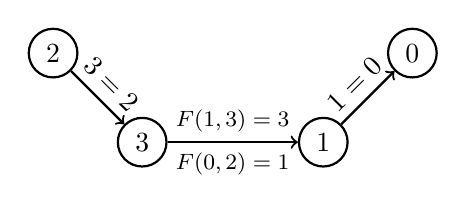
\begin{tikzpicture}[node distance={16mm}, thick, main/.style = {draw, circle}]
            \node[main] (0) {0};
            \node[main] (1) [below left of=0] {1};
            \node[main] (3) [left of=1, node distance=23mm] {3};
            \node[main] (2) [above left of=3] {2};

            \draw[->] (2) -- node[midway, above, sloped]{$3 = 2$} (3);
            \draw[->] (1) -- node[midway, above, sloped]{$1 = 0$} (0);
            \draw[->] (3) -- node[midway, above, sloped]{\footnotesize $F(1,3) = 3$} node[midway, below, sloped]{\footnotesize $F(0,2) = 1$} (1);
            \end{tikzpicture}
        \end{tabular}
    &
        \begin{tabular}{ c }
            \emph{use list}\\
            \begin{tabular}{ |c|c| }
                \hline
                index & use list \\
                \hline
                0 & [$F(0,2) = 1$, \\&$F(0,2) = 1$] \\
                \hline
           \end{tabular}
        \end{tabular}
        \begin{tabular}{ c }
            \emph{lookup table}\\
            \begin{tabular}{ |c|c| }
                \hline
                    & 0  \\
                \hline
                0 & $F(0,2) = 1$ \\
                \hline
            \end{tabular}
         \end{tabular}
    \end{tabular}
\end{table}

After the entire operation was executed, all the elements are contained in the same equivalence class.

\end{exmp}

\clearpage



The function \lstinline{are_congruent} returns \emph{True} if an equation is in the congruence closure of all the input equations so far. It simply checks if the elements have the same representative. In the case of equations containing $F$, it verifies if they have the same representative as the corresponding entry in lookup.

\begin{lstlisting}
fun are_congruent :: "congruence_closure ⇒ equation ⇒ bool"
  where
"are_congruent ⦇cc_list = l, use_list = u, lookup = t, pending = pe, proof_forest = pf, pf_labels = pfl, input = ip⦈ (a ≈ b) =
    (rep_of l a = rep_of l b)"
| "are_congruent ⦇cc_list = l, use_list = u, lookup = t, pending = pe, proof_forest = pf, pf_labels = pfl, input = ip⦈ (F a$_1$ a$_2$ ≈ a) =
    (case lookup_entry t l a$_1$ a$_2$ of
      Some (F b$_1$ b$_2$ ≈ b) ⇒ (rep_of l a = rep_of l b)
    | None ⇒ False
)"
\end{lstlisting}

\section{Proofs}

\subsection{Invariants}

At this point we can already prove some properties of the congruence closure data structure. Our approach this time is different than the one for the union-find algorithm. Instead of defining an induction rule as for the union-find proofs and prove the properties through the induction rule, we define the properties as invariants and then prove that they remain invariant after applying \lstinline|merge|. For each invariant, we need to follow the same steps. They are listed here in order to introduce a name for each step:

\begin{enumerate}
	\item Prove that the invariant holds for the initial empty congruence closure.

	\item Prove that if the invariant holds before the \lstinline|merge| operation, it also holds after the \lstinline|merge| operation. It includes the following intermediate steps:
    \begin{enumerate}
        \item The invariant holds after one step in the \lstinline{propagate_loop}. We shall refer to the two cases of the function as \lstinline{loop1} and \lstinline{loop2}.
    	\item The invariant holds after the entire \lstinline{propagate_loop}.
    	\item The invariant holds for the parameters of \lstinline{propagate_loop} in \lstinline{propagate_step}. We shall refer to this case as \lstinline{mini_step}.
    	\item It holds after \lstinline{propagate_step}.
    	\item It holds after \lstinline{propagate}.
    	\item And finally, it holds after \lstinline{merge}.
    \end{enumerate}
\end{enumerate}

Let us now look at the concrete invariants. Each list in the data structure has an invariant, which states that all the elements which are in the list are in bounds. The corresponding proofs are easy if we assume that all the input equations contain only valid elements.

One of the invariants is the usual \lstinline{ufa_invar} that we know from the union-find algorithm. The \lstinline{ufa_invar} holds for the \lstinline{cc_list} and the \lstinline{proof_forest}. These two are only modified before entering the \lstinline{mini_step}, and we already proved previously that the \lstinline{ufa_invar} holds after \lstinline{ufa_union} (in Section \ref{section:uf-isabelle}) and after \lstinline{add_edge} (Subsection \ref{subsubsection:addedge}). Therefore it also holds after \lstinline{merge}.

We define a new invariant \lstinline{same_eq_classes_invar}, which states, as the name suggests, that the union-find forest and the proof forest represent the same equivalence classes:

\begin{lstlisting}
rep_of l i = rep_of l j ⟷ rep_of pf i = rep_of pf j.
\end{lstlisting}

This invariant is important for the proofs that consider \lstinline{add_edge}. This is because we only showed that \lstinline{add_edge pf x y} terminates if \lstinline{rep_of pf x ≠ rep_of pf y}. \lstinline{propagate} only executes \lstinline{add_edge} when \lstinline{rep_of l x ≠ rep_of l y}. The invariant shows that these two statements are equivalent, therefore \lstinline{add_edge} always terminates when used inside of the algorithm.
In order to prove the invariant, given that the two lists $l$ and $pf$ are only modified during the \lstinline{mini_step}, it is sufficient to show that \lstinline{ufa_union l x y} and \lstinline{add_edge pf x y} have the same behaviour, which is what we showed in Subsection \ref{subsubsection:addedge}.

Furthermore, there is an invariant \lstinline|use_list_invar|, which states that for each representative $a$, its use list only contains equations of the type $F(b_1, b_2) = b$, where $a$ is the representative of either $b_1$ or $b_2$.

\begin{proof}
We prove that \lstinline|use_list_invar| is an invariant.
For the correctness proof after the \lstinline{propagate_loop}, we need to add an additional assumption that the second parameter only contains equations of the type $F(a_1, a_2) = a$ and the representative of either $a_1$ or $a_2$ is $rep\_of(l, b)$ (where $b$ is the right side of the equation which is being propagated). This follows from the facts that the second parameter of \lstinline{propagate_loop} is $u ! rep\_of(l, a)$, the invariant holds before the \lstinline{propagate_loop} and the new representative of $a$ after the union is $rep\_of(l, b)$.

With this assumption we can show that each time an equation gets added to the use list in the \lstinline{propagate_loop}, it is a valid equation.

In the proof after the \lstinline{merge} operation, the use list is only modified in the third case of the function and only equations of the form $F(a_1, a_2) = a$ are added to $rep\_of(l, a_1)$  and $rep\_of(l, a_2)$. Therefore all the necessary properties hold for these new equations.

For the remaining cases, the use list is either unchanged, or something is removed from it, therefore the invariant trivially holds.
\end{proof}

The invariant \lstinline|lookup_invar| for lookup is similar, it states that each entry in the lookup table at index $(i, j)$, for representatives $i$ and $j$, is either \lstinline{None} or is an equation of the form $F(a_1, a_2) = a$ where the representative of $a_1$ is $i$ and the representative of $a_2$ is $j$.

\begin{proof}
We prove that \lstinline|lookup_invar| is an invariant.
Each time an equation is added to lookup, it has the desired form and it is added to the index $(rep\_of(l, a_1), rep\_of(l, a_2))$. This happens in the \lstinline{propagate_loop} and in \lstinline{merge}. In the \lstinline{propagate_loop}, the added equation derives from the use list, for which we proved with the previous invariant that its equations have the desired form. In \lstinline|merge|, only the equations of the type $F(a_1, a_2) = a$ are added to lookup.
\end{proof}

For pending, the invariant \lstinline|pending_invar| states that the equations are either of the form \lstinline{One} ($a = b$) or \lstinline{Two} ($F(a_1, a_2) = a$) ($F(b_1, b_2) = b$) where $rep\_of(l, a_1) = rep\_of(l, b_1)$ and $rep\_of(l, a_2) = rep\_of(l, b_2)$:

\begin{proof}
We prove that \lstinline|pending_invar| is an invariant.
We need to show that in the \lstinline{propagate_loop} the equation $u1$ that we add to pending has a valid form. We know that $u1$ derives from the use list, therefore it is of the form $F(a_1, a_2) = a$. Then the lookup entry at the index $(rep\_of(l, a_1), rep\_of(l, a_2))$ is linked to it. From the lookup invariant we know that there is an entry of the form $F(b_1, b_2) = b$ at this index where $rep\_of(l, a_1) = rep\_of(l, b_1)$ and $rep\_of(l, a_2) = rep\_of(l, b_2)$. This shows that they are valid equations for pending.

The proof is analogous for the equations added to pending in \lstinline{merge}.
\end{proof}

An equivalent invariant holds for the labels in \lstinline|pf_labels|. They are only modified in \lstinline|propagate_step|, where the added label comes from \lstinline|pending|.
Therefore, the invariant follows from \lstinline|pending_invar|. This invariant is called \lstinline|pf_labels_invar|.

There is also an invariant which states that the \lstinline{cc_list}, the first dimension of the use list, both dimensions of lookup, the proof forest and the \lstinline{pf_labels} have the same length. This was trivial to prove, given that the algorithm never changes the length of the lists, and initially the lists have the same length.

The remaining invariants will be described at a later point, when they become relevant.

\subsection{Abstract Formalization of Congruence Closure}
\label{subsection:abstraction}

In order to prove the correctness of the algorithm, we define an abstraction of congruence closure. We cannot use any previously defined definitions, because the data structure that we use can only represent a subset of all possible equations, for example, it cannot represent equations of the type $a = F(b, c)$ or $F (F (a, b), c) = d$. For this reason, we define an inductive set which represents the congruence closure of a set of equations and only uses our restricted definition of equation.

\begin{lstlisting}
inductive_set Congruence_Closure :: "equation set ⇒ equation set" for S
  where
    base: "eqt ∈ S ⟹ eqt ∈ Congruence_Closure S"
  | reflexive: "(a ≈ a) ∈ Congruence_Closure S"
  | symmetric: "(a ≈ b) ∈ Congruence_Closure S
    ⟹ (b ≈ a) ∈ Congruence_Closure S"
  | transitive1: "(a ≈ b) ∈ Congruence_Closure S
    ⟹ (b ≈ c) ∈ Congruence_Closure S
    ⟹ (a ≈ c) ∈ Congruence_Closure S"
  | transitive2: "(F a$_1$ a$_2$ ≈ b) ∈ Congruence_Closure S
    ⟹ (b ≈ c) ∈ Congruence_Closure S
    ⟹ (F a$_1$ a$_2$ ≈ c) ∈ Congruence_Closure S"
  | transitive3: "(F a$_1$ a$_2$ ≈ a) ∈ Congruence_Closure S
    ⟹ (a$_1$ ≈ b$_1$) ∈ Congruence_Closure S ⟹ (a$_2$ ≈ b$_2$) ∈ Congruence_Closure S
    ⟹ (F b$_1$ b$_2$ ≈ a) ∈ Congruence_Closure S"
  | monotonic: "(F a$_1$ a$_2$ ≈ a) ∈ Congruence_Closure S
    ⟹ (F a$_1$ a$_2$ ≈ b) ∈ Congruence_Closure S
    ⟹ (a ≈ b) ∈ Congruence_Closure S"
\end{lstlisting}

The following proof rule follows directly from the definition of congruence closure. It can be used to prove equality between congruence closures of the two sets $A$ and $B$. It states that it is sufficient to prove that all elements of set $A$ are in the congruence closure of $B$ and vice versa, instead of having to prove that all elements of the congruence closure of $A$ are in the congruence closure of $B$.

\begin{lstlisting}
lemma Congruence_Closure_eq:
  assumes "⋀ a. a ∈ A ⟹ a ∈ Congruence_Closure B"
    "⋀ b. b ∈ B ⟹ b ∈ Congruence_Closure A"
  shows "Congruence_Closure A = Congruence_Closure B"
\end{lstlisting}

\subsection{Correctness}
\label{subsection:uf-correctness}

To prove that the congruence closure implementation is correct, we show that it is sound and complete,
that is, \lstinline{are_congruent cc eq} returns \emph{True} if and only if the equation $eq$ lies in the congruence closure of the input equations.

\begin{lstlisting}
theorem are_congruent_correct:
  assumes "cc_invar cc" "pending cc = []"
  shows "eq ∈ Congruence_Closure (input cc) ⟷ are_congruent cc eq"
\end{lstlisting}

The paper by Nieuwenhuis et al. \cite{Nieuwenhuis} proves this by stating the folllowing invariant which holds throughout the algorithm. We will call it the \lstinline|correctness_invar|:

\begin{lstlisting}
Congruence_Closure(representativeE ∪ pending) = Congruence_Closure input
\end{lstlisting}

where \lstinline{representativeE} can be seen as the set of equations derived from our union-find list and the equations in lookup. It is the union of the following two sets:

\begin{itemize}
    \item\lstinline{cc_list_set}, which is defined such that its congruence closure contains all the equations between two elements which have the same representative.
    \item\lstinline{lookup_entries_set} is the set of all the entries in lookup at indexes which are representatives.
\end{itemize}

\begin{lstlisting}
abbreviation cc_list_set :: "nat list ⇒ equation set"
  where
    "cc_list_set l ≡ {a ≈ rep_of l a |a. l ! a ≠ a}"
\end{lstlisting}

\begin{lstlisting}
abbreviation lookup_entries_set :: "congruence_closure ⇒ equation set"
  where
    "lookup_entries_set cc ≡ {F a' b' ≈ rep_of (cc_list cc) c | a' b' c c$_1$ c$_2$.
                      cc_list cc ! a' = a' ∧ cc_list cc ! b' = b'
                      ∧ lookup cc ! a' ! b' = Some (F c$_1$ c$_2$ ≈ c)}"
\end{lstlisting}

\begin{lstlisting}
definition representativeE :: "congruence_closure ⇒ equation set"
  where
    "representativeE cc = cc_list_set (cc_list cc) ∪ lookup_entries_set cc"
\end{lstlisting}

The formal definition of the \lstinline|correctness_invar| is the following, where \lstinline{pending_set} converts the pending list to a set of equations of the type $a = b$:

\begin{lstlisting}
definition correctness_invar :: "congruence_closure ⇒ bool"
  where
    "correctness_invar cc ≡
Congruence_Closure (representativeE cc ∪ pending_set (pending cc)) = Congruence_Closure (input cc)"
\end{lstlisting}

The set of input equations is only modified by the \lstinline{merge} function, but remains constant throughout the \lstinline{propagate} function, therefore for the proof we just need to show that the congruence closure of the \lstinline{representativeE} set and \lstinline|pending| remain unchanged after the \lstinline{propagate} function.

The main challenge is to prove that the invariant holds after the \lstinline{mini_step}. We will show that the set \lstinline{Congruence Closure (representativeE ∪ pending)} before the \lstinline{propagate_step} is equal to \lstinline{Congruence Closure (representativeE ∪ pending ∪ (u ! rep_of l a))} after the \lstinline{mini_step}.
Then we prove that the latter is equal to \lstinline{Congruence Closure (representativeE ∪ pending)}  after the \lstinline{propagate_loop}.
These two lemmas imply that the congruence closure of the \lstinline{representativeE} set and pending remain unchanged after the \lstinline{propagate} function.

We will first prove the second statement, given that it is much easer to show.

\begin{proof}
We need to show that
\lstinline{Congruence Closure (representativeE ∪ pending ∪ (u ! rep_of l a))}
before the
\lstinline{propagate_loop} is equal to the
\lstinline{Congruence Closure (representativeE ∪ pending)}  after the \lstinline{propagate_loop}.
Note that \lstinline|u| denotes the use list.
In each step of the loop, one element from $u ! rep\_of(l, a)$ is moved either to pending or to lookup. Therefore after the loop each element of $u ! rep\_of(l, a)$ is either in \lstinline|pending| or in \lstinline|representativeE|. The elements of \lstinline|pending| and \lstinline|representativeE| are never removed from the set, therefore they are present also after the loop.
\end{proof}

The first lemma is more difficult to prove. The following is the statement of the lemma. It states that the set \lstinline{Congruence Closure (representativeE ∪ pending)} before the \lstinline{propagate_step} is equal to \lstinline{Congruence Closure (representativeE ∪ pending ∪ (u ! rep_of l a))} after the \lstinline{mini_step}.

\begin{lstlisting}[label=lst:correctness_invar_mini_step]
lemma correctness_invar_mini_step:
  assumes  "a = left eq" "b = right eq"
  "cc_invar ⦇cc_list = l, use_list = u, lookup = t, pending = (eq # pe),
  proof_forest = pf, pf_labels = pfl, input = ip⦈"
     shows "Congruence_Closure
(representativeE
⦇cc_list = l, use_list = u, lookup = t, pending = (eq # pe),
proof_forest = pf, pf_labels = pfl, input = ip⦈
∪ pending_set (eq # pe))
=
Congruence_Closure (representativeE
⦇cc_list = ufa_union l a b,
    use_list = u[rep_of l a := []],
    lookup = t,
    pending = pe,
    proof_forest = add_edge pf a b,
    pf_labels = add_label pfl pf a eq,
    input = ip⦈
∪ pending_set pe
∪ set (u ! rep_of l a))"
\end{lstlisting}

\begin{proof}
There are two inclusions which need to be shown. We can use the proof rule \lstinline{Congruence_Closure_eq} from Subsection \ref{subsection:abstraction}, therefore it is sufficient to show that each equation in the set on the left-hand side is in the congruence closure of the right-hand side and vice versa. Note that the equation $eq$ of the left hand side is equal to $a = b$, because of the first two assumptions.

"$\subseteq$" It needs to be shown that the equations in the \lstinline{cc_list_set}, in lookup and in pending are in the Congruence Closure of the right-hand side.

Regarding the \lstinline{cc_list_set}, all the elements which had the same representative before a union also have the same representative after a union, therefore the equations are also present in the right hand side.

For the pending set, we need to prove that the equation that is removed from pending is still in the congruence closure after the \lstinline{mini_step}. This holds, because the equation which is removed is $a = b$, and $a$ and $b$ are in the same equivalence class after the \lstinline{ufa_union}.

The more problematic cases are the equations in lookup. After the union, $rep\_of(l, a)$ is not a root anymore, therefore the entries in lookup which have as first or second index $rep\_of(l, a)$ are not in the \lstinline{lookup_set} anymore.
The goal is to prove that these entries are exactly the equations which are present in $u ! rep\_of(l, a)$. Until now it was only proven that the equations in the use list are valid, not that they are exhaustive.
For this, we introduce a new invariant \lstinline{use_list_invar2}.
It states that all elements that are present in the lookup table at index $(i, j)$ are also in the corresponding use lists of $i$ and $j$. The invariant will be described later on.

"$\supseteq$" We need to show that the equations of the \lstinline{cc_list_set}, \lstinline{lookup_entries_set}, pending set and of $u ! rep\_of(l, a)$ on the right-hand side are in the congruence closure of the left-hand side.

The \lstinline{cc_list_set} contains equations of the form $c = rep\_of (ufa\_union(l, a, b), c)$ for each element $c$ which is not a root.
If the representative of $c$ after the union is the same as before the union, the same equation is in the \lstinline{cc_list_set} of the left-hand side.
The only representative that is different than before the union is the representative of $a$, which has as new representative $rep\_of(l, b)$.
The left-hand side contains the equations $b = rep\_of(l, b)$ and $a = b$ (which is in pending).
By transitivity, the congruence closure also contains $a = rep\_of(l, b)$ and $rep\_of(l, b)$ is the same as $rep\_of (ufa\_union(l, a, b), a)$.

Regarding lookup, all the elements which are roots after the union, are also roots before the union, therefore all elements in the \lstinline{lookup_entry_set} of the right-hand side are also in the left-hand side.

It is evident that the equations in pending on the right-hand side are also in pending in the left-hand side.

It is more difficult to show that the equations in $u ! rep\_of(l, a)$ are also present in the lookup table of the left-hand side. As before, we introduce a new invariant \lstinline{lookup_invar2}. It states that all equations that are in the use list of a root are also present in the lookup table.
\end{proof}

We introduce two new invariants of this form:
\begin{itemize}
    \item \lstinline{lookup_invar2} states that the elements in the lookup table are also present in the use list.
	\item \lstinline{use_list_invar2} states that the elements in the use list are also present in the lookup table.
\end{itemize}

Unfortunately, these two invariants do not hold in this exact form. If there are two different equations $F(a_1,a_2) = a$ and $F(b_1, b_2) = b$, with $rep\_of(l, a_1) = rep\_of(l, b_1)$ and $rep\_of(l, a_2) = rep\_of(l, b_2)$, then they cannot both be present in the lookup table, because it only stores one equation for each pair of representatives. In fact, the set of equations in lookup and in the use list are not exactly the same, but for each equation in one of them, there is a ``similar'' equation in the other one.

The difficulty was to find a suitable definition of ``similar'' which is not too strong, otherwise it wouldn't be true, but also not too weak, otherwise it is not possible to finish the proof for the invariant \lstinline{correctness_invar}.

The right definition of ``similar'' turned out to be the following:

\begin{definition}
Two equations $F(a_1, a_2) = a$ and $F(b_1, b_2) = b$ are \emph{similar}, if
\begin{enumerate}[label=(\roman*)]
\itemsep0em
    \item $rep\_of(l, a_1) = rep\_of(l, b_1)$,
    \item $rep\_of(l, a_2) = rep\_of(l, b_2)$,
    \item $(a=b) \in Congruence\_Closure (cc\_list\_set \cup pending)$.
\end{enumerate}
\end{definition}

Simply stating that $a$ and $b$ have the same representative would be too strong, because during the \lstinline|propagate| function, they are added to pending in order to be merged later, but they are not merged yet. If we use \lstinline{representativeE} instead of \lstinline{cc_list_set}, the invariant is not strong enough in order to prove \lstinline{correctness_invar_mini_step}.

The final invariants are the following:
\begin{itemize}
    \item \lstinline{lookup_invar2}: For each equation in lookup at the index $(i, j)$ (where $i$ and $j$ are representatives) there is a \emph{similar} equation in use list $i$ and one in use list $j$.
	\item \lstinline{use_list_invar2}: For each equation $F(c_1, c_2) = c$ in use list at the index $i$ (where $i$ is a representative) there is a \emph{similar} equation in lookup at the index $(rep\_of(l, c_1), rep\_of(l, c_2))$.
\end{itemize}

Here follows the proof for \lstinline{lookup_invar2}:

\begin{proof}
We need to show that if the invariant \lstinline{lookup_invar2} holds before \lstinline{merge}, then it also holds after the execution of \lstinline|merge|.

The main aim is to show that it holds after \lstinline{propagate}.
We assume that before \lstinline{propagate} the invariants \lstinline{lookup_invar2} and \lstinline{use_list_invar2} hold.
In particular, we observe that for each equation $F(c_1, c_2) = c$ in $u ! rep\_of(l, a)$, which we shall refer to as $u_a$, there is a similar equation in lookup at the index $(rep\_of(l, c_1), rep\_of(l, c_2))$.
Hence, there are similar equations in $u ! rep\_of(l, c_1)$ and in $u ! rep\_of(l, c_2)$.

In the \lstinline{mini_step}, $u_a$ is emptied, while the other use lists are not modified. Then, $u_a$ is handed over as a parameter to the \lstinline{propagate_loop}.

From now on let $l$ be the \lstinline{cc_list} after the \lstinline{ufe_union}.
In \lstinline{loop1} the lookup table and the use lists are not modified, thus there is nothing to show.

In \lstinline{loop2} we take an equation $u1$ of the form $F(c_1, c_2) = c$ from $u_a$.
The equation $u1$ is then added to lookup at the index $(rep\_of(l, c_1), rep\_of(l, c_2))$. We need to show that after this step, an equation similar to $u1$ is present both in the use list of $rep\_of(l, c_1)$ and the use list of $rep\_of(l, c_2)$.

Earlier, we observed that this was true before \lstinline{loop2}. The only use list which was modified in this step is $u_a$. Therefore the claim holds if none of those two use lists are $u_a$.

If one (or both) of the use lists are $u_a$, then the representative of the corresponding element was $rep\_of(l,a)$ before the union, therefore after the union it is $rep\_of(l,b)$. Given that $u1$ is also added to $u ! rep\_of(l, b)$ by the function, we can conclude that there is a similar equation also in this use list.
\end{proof}

Here follows the proof for \lstinline{use_list_invar2}:

\begin{proof}
We need to show that if the invariant \lstinline{use_list_invar2} holds before \lstinline{merge}, then it also holds after the execution of \lstinline|merge|.

The main challenge of this proof was to show that it holds after the \lstinline|mini_step|.
The \lstinline|mini_step| performs a \lstinline|ufa_union| and afterwards $rep\_of(l, a)$ is not a root anymore.
Therefore, if there are some equations $F(c_1, c_2) = c$ in the use list, where the representative of $c_1$ or $c_2$ is $rep\_of(l,a)$, they have a new representative after the union. Due to this, the corresponding \emph{similar} equations in the lookup table are not at the right index anymore.

We shall again refer to $u ! rep\_of (l, a)$ as $u_a$.
In the \lstinline{mini_step}, $u_a$ is emptied.
If $F(c_1, c_2) = c$ was in $u_a$, then it is removed from the use list after the \lstinline|mini_step|. In this case, the invariant holds trivially.
If $c_1$ and $c_2$ are both not in the same equivalence class as $a$, then the corresponding lookup entry has not changed and the invariant holds.
However, there could be equations in the use list at an index which is not $rep\_of(l, a)$, where $c_1$ or $c_2$ has the same representative as $a$. These equations do not have a \emph{similar} equation in lookup after the \lstinline{mini_step}, but we know from \lstinline{lookup_invar2} that they have a similar equation in $u_a$.
Therefore, in order show that \lstinline{use_list_invar2} holds after the \lstinline{propagate_loop}, it is sufficient to show that for each equation in $u_a$ a similar equation is added (or already present) in the lookup table after the \lstinline{propagate_loop}.

From now on let $l$ be the \lstinline{cc_list} after the \lstinline{ufe_union}.
The \lstinline{propagate_loop} removes an equation $F(c_1, c_2) = c$ from $u_a$, and it enters \lstinline{loop1} when lookup contains an equation $F(d_1, d_2) = d$ at the index $(rep\_of(l, c_1), rep\_of(l, c_2))$.
Then the equation $c = d$ is added to pending. Note that $F(c_1, c_2) = c$ and $F(d_1, d_2) = d$ are similar at this point, because $rep\_of(l, c_1) = rep\_of(l, d_1)$ and $rep\_of(l, c_2) = rep\_of(l, d_2)$ follows from the \lstinline{lookup_invar}, and $c = d$ is added to pending.
This case is exactly the reason why we can only prove that there is a \emph{similar} equation in lookup, and not exactly the same.

Regarding \lstinline{loop2}, it is entered when lookup contains \lstinline{None} at the index
$(rep\_of(l, c_1),$ $rep\_of(l, c_2))$. Then $F(c_1, c_2) = c$ is added to $u ! rep\_of(l, b)$ and to lookup. Obviously, an equation is \emph{similar} to itself, therefore, after this, lookup contains a similar equation to $F(c_1, c_2) = c$.
\end{proof}

With these two invariants the proof for \lstinline{correctness_invar} is completed.
The proof for \lstinline{are_congruent_correct} follows from the \lstinline{correctness_invar} and the definition of \lstinline|are_congruent|, because
the pending list is always empty after the termination of \lstinline|propagate|.

All the invariants are put together in the invariant \lstinline{cc_invar}, and using all the previously described proofs about the invariants, we can prove that \lstinline{cc_invar} holds for the initial empty data structure and that it holds after \lstinline{merge}.

\begin{lstlisting}
theorem cc_invar_initial_cc: "cc_invar (initial_cc n)"
\end{lstlisting}

\begin{proof}
All the above-mentioned invariants hold trivially for the initial case, due to the fact that all the data structures are empty or contain only \lstinline{None} in the beginning.
\end{proof}

\begin{lstlisting}
theorem cc_invar_merge:
  assumes "cc_invar cc"
  shows "cc_invar (merge cc eq)"
\end{lstlisting}

\begin{proof}
We already proved for each individual invariant that they hold after \lstinline|propagate|.
The proof for \lstinline|merge| uses the fact that \lstinline{propagate} terminates, which will be proven in the following section.
\end{proof}

\subsection{Termination}\label{section:termination-propagate}

We already proved that the functions \lstinline|add_edge| and \lstinline|add_label| terminate and the only missing proof is the termination of \lstinline|propagate|. All the remaining functions are simple enough for Isabelle to prove their termination automatically.

In order to prove the termination of \lstinline{propagate}, we show that the number of equivalence classes strictly decreases in each step of \lstinline{propagate}, therefore the function terminates at the latest when all the elements belong to the same equivalence class.

The number of equivalence classes is defined as the number of roots in the union-find forest. The \lstinline|root_set| is the set of all roots. The function \lstinline|card| returns the cardinality of a set.

\begin{lstlisting}
abbreviation root_set
  where
    "root_set l ≡ {i | i. i < length l ∧ l ! i = i}"

definition nr_eq_classes :: "nat list ⇒ nat"
  where
    "nr_eq_classes l = card (root_set l)"
\end{lstlisting}

With this, we can show that after a union, $rep\_of (l, a)$ is not a root anymore, therefore there is one less root in the forest.

\begin{lstlisting}
lemma ufa_union_decreases_nr_eq_classes:
  assumes "ufa_invar l" "a < length l"
    "rep_of l a ≠ rep_of l b"
  shows "nr_eq_classes (ufa_union l a b) = nr_eq_classes l - 1"
\end{lstlisting}

The termination proof for \lstinline{propagate} follows from this lemma, with an additional assumption that there is at least one variable, so that there is at least one equivalence class.

\begin{lstlisting}
lemma propagate_domain:
  assumes "cc_invar cc" "nr_vars cc > 0"
  shows "propagate_dom cc"
\end{lstlisting}

\begin{proof}
We prove it by induction on the amount of equivalence classes in the union-find forest.

If the pending list is empty, the function terminates. Otherwise, the first element $eq$ is taken from the pending list. We define $a$ as \lstinline{left eq} and $b$ as \lstinline{right eq}, as in the definition of the \lstinline|propagate| function.

If $a$ and $b$ are already in the same equivalence class, then the union-find list is not modified, therefore we cannot use the induction hypothesis. Therefore we apply an induction on the length of the pending list.

If $a$ and $b$ are not in the same equivalence class, they are merged by the function \lstinline{propagate_step}, therefore the number of equivalence classes decreases by one according to the lemma \lstinline{ufa_union_decreases_nr_eq_classes} and we can prove the goal by using the induction hypothesis.
\end{proof}

\chapter{The CC\_Explain Operation}\label{chapter:cc-explain}


We will implement the \emph{cc\_explain} operation for congruence closure, leaving the formal proof of correctness open for future work. This section describes the implementation, a validity and a termination proof and a proposal of how the correctness could be proven.

The \emph{cc\_explain} operation is analogous to the \emph{explain} operation for union-find. For two constants $a$ and $b$ that are congruent, it returns the subset of input equations which explain why $a$ and $b$ are congruent.

\section{Implementation}

The function \lstinline{cc_explain} has three parameters: two constants and the congruence closure data structure.
It assumes that the two constants are congruent in the data structure and returns the set of input equations which caused these two constants to be congruent. The algorithm finds the path in the proof forest between the two constants and returns the labels of the edges on the path. For each edge labeled with two equations $F(a_1, a_2) = a$ and $F(b_1, b_2) = b$, we need to also add to the output the explanation for $a_1 = b_1$ and $a_2 = b_2$. Therefore the function recursively calls the \lstinline{cc_explain} function with the parameters $(a_1, b_1)$ and $(a_2, b_2)$. In order to avoid adding redundant equations to the output, there is an additional union-find data structure. The additional union-find is local to the \lstinline{cc_explain} operation and it keeps track of the equations that are already part of the output.

We use an accumulating parameter in order to store the additional union-find. The function \lstinline|cc_explain| is a wrapper function, which hides the accumulating parameter. The actual work is done in the function \lstinline|cc_explain_aux|.
It has three parameters: the congruence closure data structure, the additional union-find and a list of pairs of constants. The output of \lstinline{cc_explain_aux} contains the explanation for all the pairs of constants in the list, except those which are already equivalent in the additional union-find. The initial union-find is a forest without edges.

\begin{lstlisting}
abbreviation cc_explain :: "congruence_closure ⇒ nat ⇒ nat ⇒ equation set"
  where
    "cc_explain cc a b ≡ cc_explain_aux cc [0..<nr_vars cc] [(a, b)]"
\end{lstlisting}

The \lstinline{cc_explain_aux} function takes one pair of elements from the list, then it
computes the lowest common ancestor between the two elements.
Afterwards, it calls the function \lstinline{explain_along_path}, which has three return values. They are named $output$, $pending$ and $new\_l$.
The $output$ is simply the set of labels on the path from the constant to the lowest common ancestor. For each edge on this path labeled with \lstinline|Two| $(F(a_1, a_2) = a)$ $(F(b_1, b_2) = b)$, the pairs $(a_1, b_1)$ and $(a_2, b_2)$ are added to the $pending$ list. The $new\_l$ is the additional union-find data structure, modified in order to keep track of the equations that are already in the output.

The following is the implementation of \lstinline|cc_explain_aux| in Isabelle.

\begin{lstlisting}
function (domintros) cc_explain_aux :: "congruence_closure ⇒ nat list
    ⇒ (nat * nat) list ⇒ equation set"
  where
    "cc_explain_aux cc l [] = {}"
  | "cc_explain_aux cc l ((a, b) # xs) =
(if are_congruent cc (a ≈ b)
then
  (let c = lowest_common_ancestor (proof_forest cc) a b;
    (output1, new_l, pending1) = explain_along_path cc l a c;
    (output2, new_new_l, pending2) = explain_along_path cc new_l b c
  in
   output1 ∪ output2 ∪ cc_explain_aux cc new_new_l (pending1 @ pending2 @ xs))
else cc_explain_aux cc l xs)"
  by pat_completeness auto
\end{lstlisting}

The additional union-find does not use \lstinline{ufa_union} for the union, instead it simply adds the same edge as the one in the proof forest.
For a more efficient implementation, the union-find can be replaced by a classical union-find data structure by showing that it has the same equivalence classes as this version.
The version used in this implementation was chosen in order to simplify the proofs.

Nieuwenhuis et al. \cite{Nieuwenhuis} also implement a $highest\_node$ function, in order to find the element of the additional union-find which is highest in the proof forest.
In our version of union-find, this corresponds to the \lstinline{rep_of} operation, because we do not use the union by rank optimization. Instead, we just make the union in the given order. When adding this optimization, a $highest\_node$ function must be also implemented.

The function \lstinline{explain_along_path cc l a c} starts at the node $a$ in the proof forest, and recursively traverses all the edges from $a$ to $c$. It skips those edges that have already been traversed sometime before in the algorithm, i.e., the edges which are present in the additional union-find $l$. Therefore it starts at the element $rep\_of(l, a)$ and considers the edge to its parent in the proof forest. It adds the label of the edge to the output and adds the edge to $l$. If necessary, it updates the pending list. The function terminates when it reaches the equivalence class of $c$ in $l$.

The following is the implementation of \lstinline|explain_along_path| in Isabelle.

\clearpage

\begin{lstlisting}
function (domintros) explain_along_path :: "congruence_closure ⇒ nat list
    ⇒ nat ⇒ nat ⇒
    (equation set * nat list * (nat * nat) list)"
  where
    "explain_along_path cc l a c =
(if rep_of l a = rep_of l c
then
  ({}, l, [])
else
  (let b = (proof_forest cc) ! rep_of l a in
    (
    case the ((pf_labels cc) ! rep_of l a) of
        One a' ⇒
          (let (output, new_l, pending) =
            explain_along_path cc (l[rep_of l a := b]) b c
          in ({a'} ∪ output, new_l, pending))
        | Two (F a$_1$ a$_2$ ≈ a') (F b$_1$ b$_2$ ≈ b') ⇒
          (let (output, new_l, pending) =
            explain_along_path cc (l[rep_of l a := b]) b c
          in
          ({(F a$_1$ a$_2$ ≈ a'), (F b$_1$ b$_2$ ≈ b')} ∪ output, new_l, [(a$_1$, b$_1$), (a$_2$, b$_2$)] @ pending))
    )
  )
)"
  by pat_completeness auto
\end{lstlisting}

\begin{exmp}
Let $cc$ be the congruence closure data structure of Example \ref{example:merge} after the \lstinline|merge| operations. We want to compute \lstinline|cc_explain cc 3 1|.

The lowest common ancestor of 3 and 1 is 1. We call the function \lstinline{explain_along_path cc l 3 1}, which considers all the edges on the path between 3 and 1. In this case it is one edge labeled $F (1,3) = 3$ and $F(0,2) = 1$. The two equations are added to the output and the pairs $(1,0)$ and $(2,3)$ are added to pending.

For the two remaining pairs in pending, the explanations contain one edge each, and the final result contains all the equations that are present in the proof forest.
\end{exmp}


The structure of the additional union-find can be formalized with an invariant, which states that all the edges in the additional union-find are also present in the proof forest. It also affirms that the \lstinline{ufa_invar} holds for the union-find list, and that the list $l$ has the same length as the \lstinline{proof_forest} list $pf$.

\begin{lstlisting}
definition explain_list_invar :: "nat list ⇒ nat list ⇒ bool"
  where
    "explain_list_invar l pf ≡ (∀ i < length l. l ! i ≠ i ⟶ l ! i = pf ! i) ∧
    (length l = length pf) ∧ ufa_invar l"
\end{lstlisting}

Each time an edge is added to the union-find in \lstinline{explain_along_path}, it is an edge which is also present in the proof forest, therefore it is easy to prove that this is an invariant.

This invariant implies the following useful lemma, which states that each path in the additional union-find is also present in the proof forest.

\begin{lstlisting}
lemma explain_list_invar_paths:
  "path l a p b ⟹ explain_list_invar l pf ⟹ path pf a p b"
\end{lstlisting}

\section{Termination}

We need to prove the termination of the two functions \lstinline{explain_along_path} and \lstinline{cc_explain_aux}.

The function \lstinline{explain_along_path} starts at the node $a$ and recursively considers the parent node until it reaches $c$. Therefore the function terminates if $c$ is an ancestor of $a$.

\begin{lstlisting}
theorem explain_along_path_domain:
  assumes "cc_invar cc"
    "explain_list_invar l (proof_forest cc)"
    "path (proof_forest cc) c p a"
  shows "explain_along_path_dom (cc, l, a, c)"
\end{lstlisting}

\begin{proof}
In the following, the arrows $\rightarrow^*$ represent paths of arbitrary length, including paths with no edges, and $\rightarrow$ represent exactly one edge.

The proof is by induction on the length of the path $p$.
If the path has length 1 or if \lstinline{rep_of l a = rep_of l c}, the function terminates immediately.

If the path is longer, then the union-find $l$ contains the following path:

$a \rightarrow^* rep\_of(l,a)$

and the proof forest $pf$ contains the same path, which continues until it reaches $c$:

$a \rightarrow^* rep\_of(l,a) \rightarrow pf ! rep\_of(l,a) \rightarrow^* c$.

Therefore there is a shorter path from $c$ to $pf ! rep\_of(l,a)$ in the proof forest and we can apply the induction hypothesis for the recursive call of \lstinline{explain_along_path}. Given that the recursive call terminates, the function also terminates.
\end{proof}

The function \lstinline{explain_along_path} is only executed in \lstinline{cc_explain_aux} when $c$ is the lowest common ancestor of $a$ and $b$, therefore the assumption that there is a path from $c$ to $a$ always holds when the function is executed.

In order to prove the termination of \lstinline{cc_explain_aux}, we use the same idea as for the termination proof of \lstinline{propagate} in Subsection \ref{section:termination-propagate}. We consider the number of equivalence classes of the additional union-find, and prove that the number of equivalence classes decreases in each call of \lstinline{explain_along_path}.

First, we prove that the number of equivalence classes decreases with a function update, if the updated index is a root:

\begin{lstlisting}
lemma list_upd_eq_classes:
  assumes "a ≠ b" "l ! a = a" "a < length l"
  shows "nr_eq_classes (l[a := b]) < nr_eq_classes l"
\end{lstlisting}

By examining the function \lstinline{explain_along_path}, we see that each time the union-find list is updated, the updated index is a root, therefore the number of equivalence classes decreases.
However, if \lstinline{rep_of l a = rep_of l c}, the union-find list is never updated, therefore we can only show that the number of equivalence classes does not increase after \lstinline{explain_along_path}:

\begin{lstlisting}
lemma explain_along_path_eq_classes:
  assumes "cc_invar cc"
    "explain_list_invar l (proof_forest cc)"
    "path (proof_forest cc) c p a"
  shows "nr_eq_classes (fst (snd (explain_along_path cc l a c))) ≤ nr_eq_classes l"
\end{lstlisting}

We can show that it strictly decreases if the pending list is not empty after the function  \lstinline{explain_along_path}, because we always update the union-find list when we add elements to pending:

\begin{lstlisting}
lemma explain_along_path_eq_classes_if_pending_not_empty:
  assumes "cc_invar cc"
    "explain_list_invar l (proof_forest cc)"
    "path (proof_forest cc) c p a"
    "snd (snd (explain_along_path cc l a c)) ≠ []"
  shows "nr_eq_classes (fst (snd (explain_along_path cc l a c))) < nr_eq_classes l"
\end{lstlisting}

With these two lemmas, we can prove that \lstinline{cc_explain_aux} terminates:

\begin{lstlisting}
theorem cc_explain_aux_domain:
  assumes "cc_invar cc"
    "explain_list_invar l (proof_forest cc)"
  shows "cc_explain_aux_dom (cc, l, xs)"
\end{lstlisting}


\begin{proof}
We show it by using a nested induction: the outer induction is on the number of equivalence classes, and the inner induction is on the length of $xs$.
If $xs$ is empty, then the function terminates.

If \lstinline{are_congruent (a ≈ b)}, then we do a case distinction: if both \lstinline{pending1} and \lstinline{pending2} are empty, then the length of $xs$ decreases and we can use the induction hypothesis of the inner induction. In this case we need the previously proven lemma \lstinline{explain_along_path_eq_classes}, because we also need to show that the number of equivalence classes does not increase. If one of the pending lists is not empty, we use \lstinline{explain_along_path_eq_classes_if_pending_not_empty} to show that the \lstinline{nr_eq_classes} has decreased, and we use the first induction hypothesis.

If \lstinline{are_congruent (a ≈ b)} does not hold, then the length of $xs$ decreases and we can use the second induction hypothesis.
\end{proof}


\section{Validity}

Similarly to the \lstinline{explain} operation for union-find (see Subsection \ref{subsection:uf-correctness}), we can prove that the equations in the output of \lstinline{cc_explain} are a subset of the input equations.

\begin{lstlisting}
theorem cc_explain_valid:
  assumes "cc_invar cc" "validity_invar cc"
  shows "cc_explain cc a b ⊆ input cc"
\end{lstlisting}

We assume the \lstinline{cc_invar} which we have previously proven, and we introduce a new invariant, the \lstinline{validity_invar}. It states that all the equations in \lstinline{pf_labels}, \lstinline{lookup}, \lstinline{use_list} and \lstinline{pending} are equations from the \lstinline{input} set. In order to show that this is an invariant, we remark that all the new equations added in \lstinline{merge} to any data structure are also added to the \lstinline{input} set. In \lstinline{propagate}, no new equations are added, instead the equations are simply moved around between different lists.

With this invariant, we can prove that the output of \lstinline{explain_along_path} is valid.

\begin{lstlisting}
lemma explain_along_path_valid:
  assumes "cc_invar cc" "validity_invar cc"
    "explain_list_invar l (proof_forest cc)"
    "path (proof_forest cc) c p a"
  shows "fst (explain_along_path cc l a c) ⊆ input cc"
\end{lstlisting}

\begin{proof}
We already proved that \lstinline{explain_along_path} terminates, therefore we can use the induction rule of the function.

If \lstinline{rep_of l a = rep_of l c}, then the output of \lstinline{explain_along_path} is the empty set, therefore the proof is trivial.

Else, the new equations added to the output derive from the proof forest, more specifically from \lstinline{(pf_labels cc) ! rep_of l a}.
The \lstinline{validity_invar} states that all edge labels are valid, that is, the entries in \lstinline|pf_labels| are valid for indexes which are not roots. If the index is a root, there is no outgoing edge, therefore those entries are not valid.
In order to use the invariant, we need to prove that $rep\_of(l, a)$ is not a root in the proof forest.
Given that we assumed that there is a path from $c$ to $a$ in the proof forest, we know that $c$ is nearer to the root than $a$ and we can show that if $rep\_of(l,a)$ was a root in the proof forest, then $c$ can only be equal to the root, therefore \lstinline{rep_of l a = rep_of l c}, which is a contradiction.
\end{proof}

From this lemma we can easily show the theorem \lstinline{cc_explain_valid} by computation induction on \lstinline{cc_explain_aux}. We can use the induction rule because we have already proven the termination of \lstinline{cc_explain_aux}.

\section{Correctness}

Proving the correctness of \lstinline{cc_explain} is more complicated than expected. The most intuitive strategy would be to use the induction rule of \lstinline{cc_explain_aux}, but it is not strong enough to prove it. Our goal is to show that the two variables are congruent under the congruence closure of the output of \lstinline{cc_explain}.

\begin{lstlisting}
theorem cc_explain_correct:
  assumes "are_congruent cc (a ≈ b)" "cc_invar cc"
  shows "(a ≈ b) ∈ Congruence_Closure (cc_explain cc a b)"
\end{lstlisting}

It is possible to show for \lstinline{explain_along_path} that $a = b$ is in the congruence closure of the output, pending and the \lstinline{representative_set l}. Intuitively, the function adds the necessary equations to output and pending, except if the elements of the equations are already in the same equivalence class in the additional union-find.

\begin{lstlisting}
lemma explain_along_path_correctness:
  assumes "explain_along_path_dom (cc, l, a, c)"
    "explain_along_path cc l a c = (output, new_l, pend)"
    "path pf c pAC a"
    "cc_invar cc"
    "explain_list_invar l (proof_forest cc)"
  shows "(a ≈ c) ∈ Congruence_Closure (cc_list_set l ∪ output
∪ pending_set_explain pend)"
\end{lstlisting}

Given that at after the termination of the function \lstinline{pending} and the initial union-find $l$ are empty, this should imply that $a = b$ is in the congruence closure of \lstinline{cc_explain}.
However, this argument is not applicable. I will illustrate this with an example.

\begin{exmp}
We consider the following proof forest:

\begin{center}
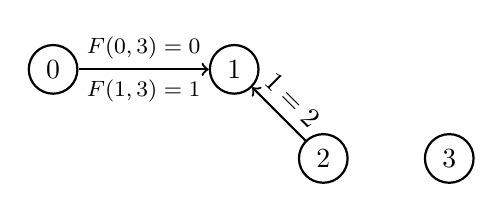
\begin{tikzpicture}[node distance={16mm}, thick, main/.style = {draw, circle}]
\node[main] (1) {1};
\node[main] (0) [left of=1, node distance=23mm] {0};
\node[main] (2) [below right of=1] {2};
\node[main] (3) [right of=2] {3};

\draw[->] (0) -- node[midway, above, sloped]{\footnotesize $F(0,3) = 0$} node[midway, below, sloped]{\footnotesize $F(1,3) = 1$} (1);
\draw[->] (2) -- node[midway, above, sloped]{$1 = 2$} (1);
\end{tikzpicture}
\end{center}

The \lstinline{cc_invar} holds, in particular \lstinline{pf_labels_invar} holds. This invariant states that for the labels in the proof forest of the type $F(a_1, a_2) = a_3$ and $F(b_1, b_2) = b_3$ it holds that $rep\_of(l, a_1) = rep\_of(l, b_1)$ and $rep\_of(l, a_2) = rep\_of(l, b_2)$.

If we call \lstinline{cc_explain cc 0 1} it terminates and returns the two equations $F(0,3) = 0$ and $F(1,3) = 1$.
However, $0 = 1$ is not in the congruence closure of these two equations.
The problem in this case is that when \lstinline{explain_along_path cc l 0 1} is called, it simply adds $(0, 1)$ to pending, adds the two equations to output and adds the edge between $0$ and $1$ to the additional union-find.
In the recursive call of the function, $(0,1)$ is taken from pending.
The algorithm sees that it has already considered this edge, and returns an empty output.
\end{exmp}

The previous example shows that the invariant \lstinline|cc_invar| together with the lemma \lstinline{explain_along_path_correctness} are not enough to prove that \lstinline{cc_explain} is correct. However, it does not show that \lstinline{cc_explain} is incorrect, because the proof forest in the example cannot be produced by subsequent merges. For the labels in the proof forest of the type $F(a_1, a_2) = a_3$ and $F(b_1, b_2) = b_3$, it not only holds that $rep\_of(l, a_1) = rep\_of(l, b_1)$ and $rep\_of(l, a_2) = rep\_of(l, b_2)$, but also that those representatives have been equal before the addition of the edge. Therefore, \lstinline{explain_along_path} will never add equations to pending which are only congruent if the output equations are congruent.

An idea for the proof would be to define an additional invariant that expresses what was explained in the previous paragraph. Alternatively, we could define the correctness of \lstinline{cc_explain} as an invariant, and prove that it is an invariant of merge.

In order to prove that it is an invariant, we need to show that after a \lstinline{merge} operation, the path between two elements remains the same in the proof forest. This implies that \lstinline{cc_explain} considers the same edges before and after the \lstinline|merge|. The difficulty with this approach is that some edges could be inverted by \lstinline{add_edge}, which means that the lowest common ancestor of two elements could also change.
In other words, the \lstinline{cc_explain} function before and after \lstinline|merge| considers the same edges but in a completely different order. As a result, we also need to show that the order of the edges which \lstinline{cc_explain} considers does not matter.